\section*{\centering ABSTRACT}

Among all forms of sculpture, bas-relief is arguably the closest to painting .  We present a new approach for generating a bas-relief from a single brush painting.We do not aim to recover exact depth of a painting, which is a tricky computer vision problem, requiring assumptions that are rarely satisfied.Instead, our approach exploits the concept of brush strokes, making each brush stroke possible to generate a correspond bas-relief proxies(depth map of strokes),used for bas-relief editing. To segment brush strokes in 2D paintings, we reformulate layer decomposition and MSERs segmentation by imposing boundary constraints, which can make strokes smooth and complete. The resulting brush strokes are sufficient to evoke the impression of the consistent 3D shapes on bas-relief, so that they may be further edited in 3D space. This fulfills the request of recomposition in bas-relief design. Currently, our research focus on brush paintings with relatively sparse and clear strokes. 


\begin{figure}[H]
\centering
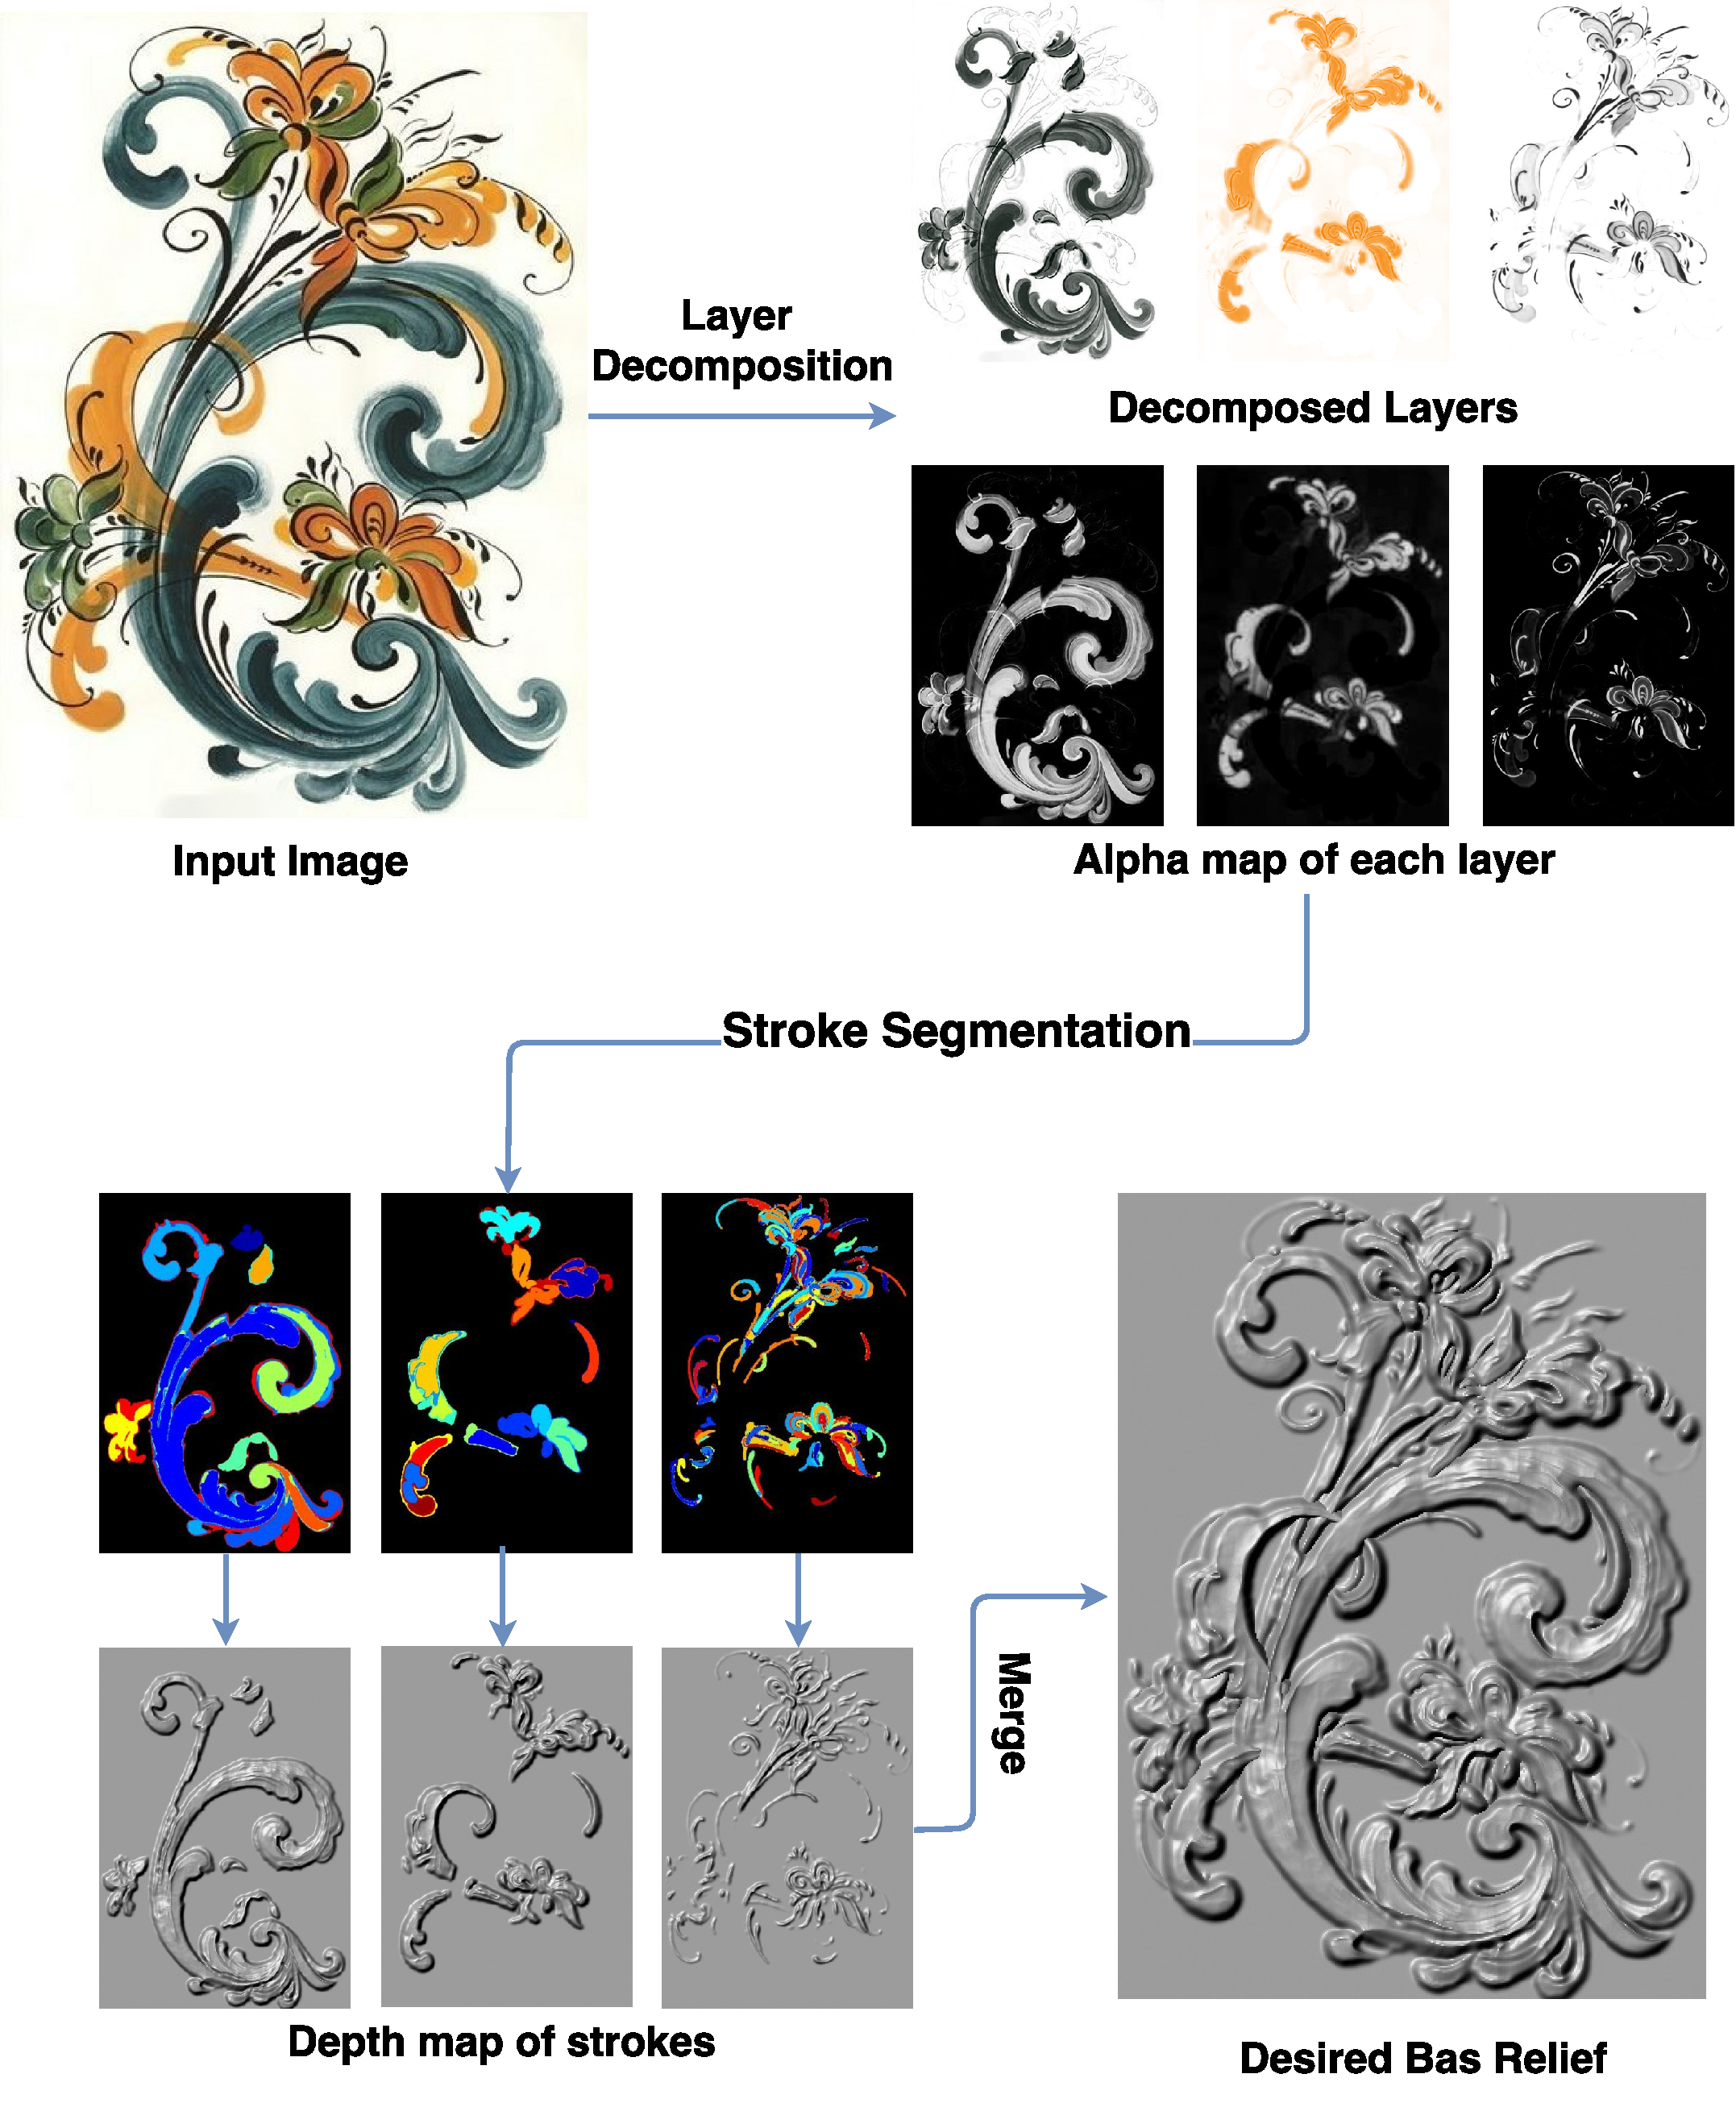
\includegraphics[scale=0.4]{overview.pdf}
\caption{Pipeline Overview}
\label{pip}
\end{figure} 
 
\newpage


 

